\chapter{Analysis and Theoretical Foundation}
\label{ch:analysis}
While the previous chapter covered existing theoretical approaches which intersect somewhat to the ATHENA approach itself, the following will go into more detail related to scientific methods used throughout the application. The theoretical foundations of ATHENA will be covered, with the conceptual behaviour of such an application being formally described. Please note that the following set of methods apply to a variety of text feature extraction use cases and are not in any way bound to the application itself, but rather belong to the general approach. For details on the implementation of the ATHENA approach as implemented in a Django/Python web application, consult Chapter 5 of this thesis.

\section{Pipeline architecture}
Pipeline architectures are an idea emerged at the dawn of the industrial era to better manage the production cycle of factories. The basic idea is that workers are specialised and only perform small parts of the total work needed to complete a task or project, with the semi-finished goods being transported between specialised stations throughout the process.

These concepts were first applied in computer sciences in the context of pipelined CPUs\footnote{Central Processing Unit} with the aim of increasing instruction number per unit of time. This meant executing the micro-instructions separately, storing the result and reusing that stored result as message exchange between the pipeline steps. Figure \ref{fig:cpupipe} presents a classical RISC pipeline with 5 steps: Instruction Fetch, Instruction Decode, Execute, Memory access and Register write back.

\begin{figure}
    \centering
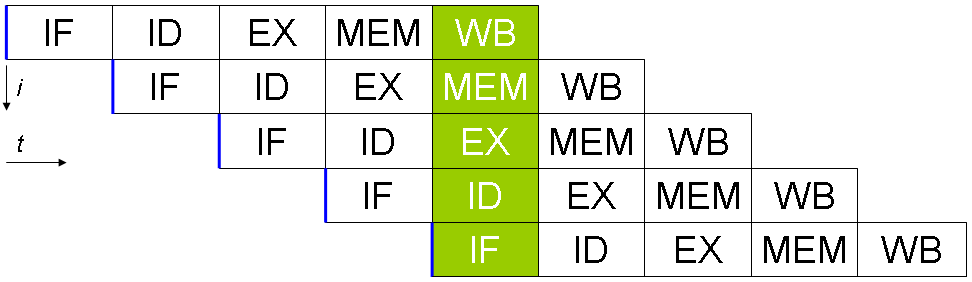
\includegraphics[width=0.8\columnwidth]{img/cpupipe.png}
    \caption{Five-stage pipeline in a RISC machine}
    \label{fig:cpupipe}
\end{figure}

As discussed in the previous chapter, the pipeline architecture has subsequently gained momentum in high-level computing as well. The pipeline architecture is suitable for projects which feature large transformation efforts with multiple failure points. By separating the set of transformations into separate steps, the black boxes composing the broken down architecture are separate entities with manageable numbers of failure points. Furthermore, the communication between the black boxes takes place by using stored semi-finished data as a method of message exchange.

Pipeline architectures are well suited for Object-Oriented Programming best practices as well, since the concept itself is SOLID (Single Responsibility, Open/Closed, Liskov Substitutional, Interface Segregated and Dependency Inverted, as per previous chapter discussion). The architecture is also encouraging of loose coupling and scaling to distributed applications. Considering the task of developing applications for fetching and analysing data from social media, it is self-understood that scaling towards distribution might be mandatory from some point on.

\subsection{Black boxes}
In the context of this approach, the black boxes which correspond to different pipeline stages are:

\begin{itemize}
\item the Harvesting module: methodology and system of fetching data from external APIs provided by different social networks.
\item the Enhancement module: methodology for enhancing the fetched and stored data with specific details which model its structure and particularities
\item the Normalisation module: handles the flattening of fetched and stored harvests using different configurations. This module helps filter outliers, noisy and/or erroneous data points, in the end storing the result.
\item the Analysis module: performs comparative analysis of differences and commonalities between already normalised data sets, with focus on differences and commonalities between the two
\end{itemize}

\subsection{Communication between modules}
The execution of the Harvesting module results in the fetching and storage of related document sets. These collections of documents are stored using a persistent and manageable data source. For the time being, the choice of the data source backend is unimportant, especially from a formal point of view. However, it must be noted that the data source to be chosen is required to be fast, scalable and easily manageable.

The communication from Harvest to Enhancement and Normalisation respectively is one much similar to the classical approach of pipelined CPUs, i.e. the data is stored and then recollected inside the destination modules. As it will be seen in further sections, the nature of asynchronous jobs (employed in order to fetch the data in rate-limited APIs) adds an extra buffer to this ad-hoc message exchange channel, by not permitting yet incomplete harvests to enter processes such as Enhancement and Normalisation.

Enhancement is a module without side-effects, which means the data it uses as part of calculations remains unchanged. However, it is another case when discussing the Normalisation module. The calculations of data flattening done by the Normalisation step are recorded in the persistence layer, for further use in the Analysis module.

Last but not least, the final step considers the data previously saved by the Normalisation step to make comparative calculations of similarity and differences between two document collections which have already passed through the Harvest and Normalisation steps and are now both:

\begin{itemize}
\item correspondent to real-life documents authored by users using the queried social network

\textbf{and}
\item flattened in order to eliminate outliers and noise.
\end{itemize}

Data is generally considered as output from source boxes (steps) and input for destination ones. This is easily enforceable using step-wise validation.

\section{Asynchronous application behaviour}
The following section covers the particularities of the Harvesting module, which necessitates special attention in regards to the execution of processes. I will cover the particularities of asynchronous jobs and why it is necessary to place part of this module inside such a job.

\subsection{Asynchronous jobs}
An important classification in regards of job execution in web applications (and not only) is whether the execution is synchronous or asynchronous. A synchronous job receives its input from the end user via the application, it executes and returns a result instantly, which the user waits for and gets immediately. In the case of asynchronous jobs, users send their input to the application, but instead of waiting for a response to come, they continue to browse, interact with the application and maybe even send more and more jobs to execute. On the backend side, said jobs are executed and might or might not notify the user when they have finished.

In dealing with large response times, it is generally better to use asynchronous execution, for a variety of reasons which culminate with the user's general experience. If a user is forced to wait for a result and prevented from doing anything else, they get easily frustrated. The ATHENA methodology, in particular the Harvest module, requires extensive querying of external data sources. Furthermore, the external APIs provided by social networks enforce rate limits, which means the client application can only get a maximum number or total size of documents before needing to sleep until the limit is replenished. It is impossible in this context to make the user wait for the result.

\subsection{Job handling with the Producer/Consumer architecture}
Up to now, we established the need for an asynchronous job execution as part of the Harvest module. To clarify on that, it is needed to establish a general architecture in which these jobs are created, executed and finalised.

\begin{figure}
    \centering
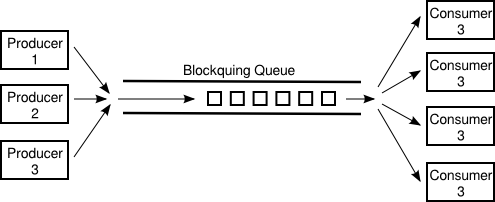
\includegraphics[width=0.8\columnwidth]{img/producer-consumer.png}
    \caption{Producer/Consumer architecture example}
    \label{fig:prodcons}
\end{figure}

The Producer/Consumer concept subsumes problems, architectures and design pattern suggestions throughout the computer science field, starting from the didactic example of the need to introduce semaphores and atomic operations in computer architecture. As a job execution framework, this setup is formalised as such:

Two processes called Producer and Consumer are connected using a buffer, which usually takes the form of a Blocking Queue. The Producer is tasked to generate data, add it into the buffer and start over. Meanwhile, the Consumer is removing data from the buffer (piecewise and in the order it was produced). In the context of asynchronous job execution, the Producer is the one that creates the jobs, while the Consumer handles each job, in order. Figure \ref{fig:prodcons} contains a graphical representation of these details.

ATHENA includes a Producer-Consumer architecture inside its Harvest pipeline, as part of the asynchronous job execution whose necessity was explained above. While the task of getting the options from an end user and creating the job setup itself should be part of a core system, the jobs are then sent via a buffer towards a Consumer. The Consumer is instructed to fetch the related document sets as per the read options from the buffer. As part of the Consumer, a social network's REST API will be used as a source for the document collection.

To clarify, the asynchronous functionality is provided by the Consumer. Indeed the buffer is also outside what we consider core synchronous functionality, but its just a passive data source.

\section{REST API communication}
As discussed in the previous chapter, social networks have not only developed in-house analysis applications, but moreover exposed APIs (Application Programming Interfaces) which developers can use in order to query for documents authored by users of that social network. Previous sections have described \emph{how} Harvesting works, but not exactly \emph{what} it does, i.e. the executable content of the Consumer.

Most APIs follow the REST architecture, which stands for Representational State Transfer. The method is widely-used as opposed to other Application service implementations, because of its compatibility between applications written in different programming languages and its general ease of use, which is based on calling URIs with one of the classical HTTP verbs:

\begin{itemize}
\item GET: to read data
\item POST: to modify data
\item PUT: to update by replacing data
\item PATCH: to update/modify data
\item DELETE: to remove data
\end{itemize}

REST services are called by a \emph{client} and affect a \emph{server}. In order to acquire data about users and posts from an API exposed by a social network, ATHENA assumes the role of a client in the exchange with the social network's servers. Usually since this approach works by fetching data and not modifying it, the primarily used verb is GET, along with different parameters.

\subsection{Authentication}
External APIs usually provide users with a variety of access tokens and/or secret codes which serve both to protect the API from illegal usage by identifying the client application and cutting off its access in case any irregularities are found. On the other hand, the client can make sure that, if they haven't distributed the access tokens to other parties, their account is safe from outside penetration, i.e. other clients can not impersonate the application to piggypack any requests.

These authentication details are usually sent in every request or otherwise the credentials are established once in a certain interval of time. In any case, for the examples below detailing the usage of HTTP methods and parameters in fetching social data, we oversee authentication description for simplicity purposes.

\subsection{Filtering with parameters}
When filtering the set of posts we are interested in, we consider input from the end user of ATHENA. They are not interested in getting all the posts of all the users in every time. However, the details provided by the user when creating the Harvesting job can be used in order to filter the request to only contain conformant data.

GET parameters can be directly added to the URL called on the server, by adding a question mark character at the end of the base URI (?) and adding key and value pairs of the desired parameters separated by ampersands (\&). The pairs themselves take the form:

\[key=value\]

ATHENA filters content by its label (content or, in the specific case of Twitter, hashtag) and date limits (start and end dates), which means the query URL will look something similar to:

\[https://api.twitter.com/1.1/search/tweets.json?\]
\[q=\#python\&since=2016-06-06\&until=2016-06-07\&lang=en\]

\subsection{API wrapper libraries}
It is worth mentioning that in often cases, the same type of requests are used by many developers. The repetitive nature of the task to be implemented creates the business value for API wrappers, which can seamlessly be used by developers, based on some input access keys and wrapper functions.

It was previously discussed throughout this thesis that external APIs usually enforce rate limits. These can usually take the form of maximum number or size of responses per unit of time. The solution is sometimes to halt the processes fetching the data until the rate limits are replenished. These is another very common use case with repetitive nature, which makes it a candidate for wrapper functions as well. In Chapter 5 we describe the activity of chosing an implementation method for these concepts, factoring in the benefits of API wrapper libraries and functions.

\section{Vectorising the data space}
As part of the Enhancement step, ATHENA is mostly concerned with structural particularities of the document sets. In other words, we are interested in modeling the most common occurrences of content, the most popular labels and categories assigned by authors and the general correspondence between users, their posted documents and their creative content.

A first step in achieving content analysis is to perform term ocurrence analysis. This step is often called \emph{vectorising} the collection of text documents, since it takes as an input the set of documents (as arrays of terms) and outputs a $m \times n$ matrix of term occurrences, where:

\begin{itemize}
\item $m$ is the number of rows i.e. text documents in the collection
\item $n$ is the number of columns i.e. tokens found (also known as terms, however the notion of token is used since the terms are intended as single-piece elements, with eventual corelations being studied later)
\end{itemize}

But what do we consider to be a token? Well, for the first iteration of this approach, the decision to use hashtags was a result of their prevalence throughout various social networks. This particular type of labeling is done directly by the user with special characters and has gained momentum ever since its introduction on Twitter, Instagram and later Facebook. Hashtags are therefore informal labels and/or categories, which transforms this otherwise unsupervised task of feature extraction into one of less difficulty, since users themselves have performed a sort of annotation.

A larger discussion about the usage of hashtags in the particular context of Twitter can be consulted in the next chapter. For now, suffice it to say that the vectorisation can consider only particular forms as tokens and can ignore non-hashtag content if instructed so.

\subsection{Sparse matrices}
Special attention needs to be dedicated to the result of the vectorisation step. Indeed the result is a matrix but considering the large number of documents and the little number of re-occurring terms one document may contain, the matrix will undoubtedly have many 0 values. Such a matrix is called \emph{sparse} and it requires special data structures and algorithms for proper processing. For example, consider the following document set:

\begin{enumerate}
\item The \#cat in the \#hat.
\item The \#hat in the \#flat.
\item The \#flat \#data set is better for \#analysis.
\end{enumerate}

Considering hashtag-only vectorisation i.e. only for tokens starting with the character "\#", it produces the following result, with columns from top to bottom: \#cat, \#hat, \#flat, \#data, \#analysis and documents from left to right 1, 2, 3:

\[ \left( \begin{array}{ccc}
1 & 0 & 0 \\
1 & 1 & 0 \\
0 & 1 & 1 \\
0 & 0 & 1 \\
0 & 0 & 1 \end{array} \right)\] 

With only 3 documents the resulting matrix is already somewhat sparse (containing 8 zero values to 7 non-zero ones), but considering a much larger document number, it becomes clear that a high proportion of the resulting matrix will contain zero values.

Generally a sparse matrix can be stored in different ways, including the classical two-dimensional array. However, traversing and modifying such a large data structure is considered cost-ineffective. Other formats\footnote{https://en.wikipedia.org/wiki/Sparse\_matrix} include those optimised for modifications:

\begin{itemize}
\item dictionary of keys: maps $(row, column)$ pairs to the value of elements
\item list of lists: stores one list per row
\item coordinate list: stores $(row, column, value)$ tuples
\end{itemize}

While other formats support efficient access and matrix operations:

\begin{itemize}
\item compressed sparse row: similar to coordinate list, but compresses the row indices. Indicated for row access and vector multiplication
\item compressed sparse column: similar to compressed sparse row but with columns compressed. Recommended for arithmetic operations and vector products
\end{itemize}

The exact type of storage used depends on the implementation itself. Some processing methods may produce one type of representation or another, but the underlying data structure will always be a sparse matrix. Having performed vectorisation, it is then a matter of calculations and choosing the correct algorithms towards the goal.

Vectorising the space and calculating clusters (as discussed below) are important parts of the Enhancement step in ATHENA.

\section{Clustering with KMeans}
While mere presence or absence of terms inside a document collection is interesting to consult, it is not a detail which gives users much information about the composition of said document collection. Vectorisation of terms is in this case a precursor for the clustering step, which uses the previously generated sparse matrix for identifying commonalities between some documents.

By clustering we generally refer to an approach, algorithm or general endeavour which assigns data points to agglomerations called clusters. The basic example follows points on a plane with given coordinates. Clusters of will be formed based on data points agglomerations, considered by the Euclidean distance measurement.

\begin{figure}
    \centering
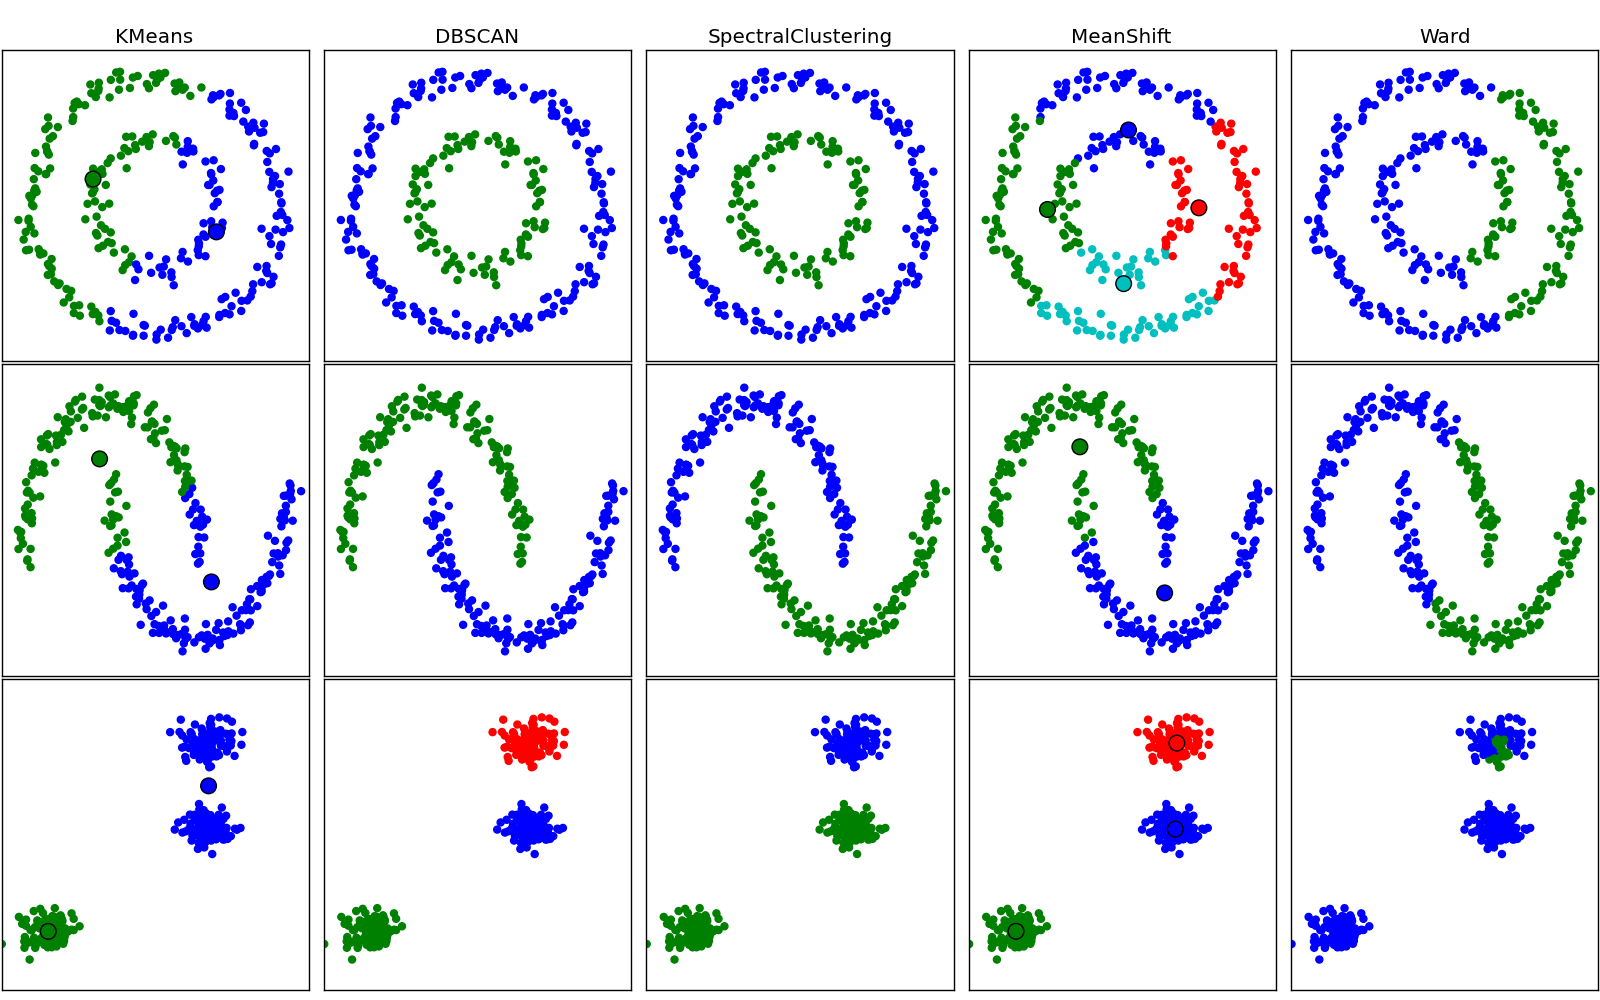
\includegraphics[width=\columnwidth]{img/clustering.png}
    \caption{Clustering algorithms in effect on various data sets}
    \label{fig:clustering}
\end{figure}

A variety of clustering algorithms exist, all with specific advantages and disadvantages. Some algorithms perform better on pattern-full data, while others handle unexpected metrics better. The efficiency of a clustering algorithm depends on the data particularities, initialisation and running options. Figure \ref{fig:clustering} exemplifies the performance of various clustering algorithms on different data sets, with data points marked as belonging to certain clusters by coloring on the graph. Note that some algorithms also place \emph{centroids} (represented in the figure as small circles) which represent the center of a cluster, although it doesn't necessarily coincide with a data point.

When considering term occurrence, clearly the distance is not the Euclidean classical one. However the distance in use here is the commonality of terms used throughout the document space. E.g. documents which are used in many documents together are considered \emph{close} while terms which never intersect inside the same document are \emph{far} from one another. Considering the general lack of irregularities and patterns possible inside a textual dataset, the K-Means algorithm is a good fit to our approach.

Essentially, the algorithm works by initialising a number of $k$ centroids and subsequently changing the cluster location and the data point assignment based on mean distances, i.e. at every execution step, a point is assigned to the closest centroid and a centroid's position is recalculated at the mean of its components. I will not go into much detail regarding the steps here, but rather into the problem of centroid initialisation and KMeans variants available.

\subsection{Centroid initialisation}
Centroid initialisation is a sensitive problem when considering K-Means algorithm implementation due to the propagation of errors and convergence time costliness an inappropriate initial setup could produce. The goal of centroid initialisation algorithms is to minimise intra-class distance (sum of Euclidean distances between each data point and its centroid). Some common centroid initialisation methods are:

\begin{itemize}
\item Forgy: randomly chooses k data points and uses them as initial means
\item Random partition: starts by randomly assigning a cluster to each data point
\item KMeans++: works by selecting an $i$ centroid using a probability function based on the minimum distance from an initial $x$. This algorithm usually prevents accidental selection of close centroids, which can propagate and affect the algorithm's working. Using a KMeans++ initialisation, it is guaranteed that the algorithm will converge in O(log k)
\end{itemize}

In order to ensure fast convergence to a good solution, the KMeans++ initialisation algorithm is a good fit for the approach presented in this thesis.\label{kmeansplusplus}

\section{Power law fitting}
In Chapter 3 I discussed the particularities of data sets which correspond to power functions. In this section I will ellaborate on the usage of these modeling techniques to identify potential pages, bots and fake accounts on social media. In concernes related to power functions and fractalic modeling, it is not problematic to output a data set corresponding to a power function, but I will present an algorithm handling the reverse problem: how, given a data set, we can calculate the degree to which it corresponds to a power law.

\subsection{Power functions and well-known examples}
\label{plfittheory}
In Chapter 3 I briefly mentioned Vilfredo Pareto's now famous law which stated that 80\% of the effects are generally the results of 20\% of actions, as well as other scientists' (such as Mandelbrot and Taleb) concerns towards understanding and modeling general power law principles. Pareto's law indeed seems to be applicable to many domains and fields of economics and computer science\footnote{https://en.wikipedia.org/wiki/Pareto\_principle}

\begin{itemize}
\item (in business) 80\% of a company's profits come from 20\% of its customers
\item (in sales) 80\% of a company's sales are made by 20\% of its sale staff
\item (in load testing, as a general recommendation for testing) 80\% of the traffic occurs in 20\% of the time
\item (in artficial intelligence) some toy-worlds have demonstrated a natural convergence towards wealth distribution of 80\%/20\%
\end{itemize}

The proportion is of course not always 80/20 as suggested in numerous studies finding even larger discrepancies in such behaviour. For example, a 2013 study \cite{muchnik2013origins} found that 80\% of content on the online user-editable encyclopedia Wikipedia is authored by a mere 5\% of Wikipedia users. This suggest that there is merit in studying the user's post numbers as being indicative of some special pattern. There is not a study formally demonstrating that abnormally frequent posters are indeed pages, bots or fake accounts, and even in ATHENA we offer the raw modeling data to end users. However, empirical evidence seems to suggest a degree of truth in this matter, at least for some users. I do believe the modern trend in analysing fat tails and power functions, as well as non-Gaussian probability distributions will continue and further investigations can be made into the subject.

\section{HashMap-based duplicate removal}
During the Normalisation step, a classical duplication removal algorithm is used. HashMaps as a general concept are data structures that behave as a dictionary of pairs (key, value). However, the interesting part is that the constraint of uniqueness can be set on such a structure, which enforces that the collection of all keys is a set. This means that no duplicate keys may be found in the same HashMap. HashMaps have different interpretations and names in different programming languages, e.g. in Ruby they are called Hashes, in Java HashSets and in Python Dictionaries.

The duplication removal algorithm loops through the existing dataset and appends the corresponding (key, value) pairs to a HashSet. In the simplest implementation, collision is simply a matter of overwriting the existent data, but other options include checking whether the key already exists, which is of $O(1)$ complexity. This means the final algorithm complexity will be $O(n)$, corresponding to the looping part.

It is important to note that the implementation itself may vary per programming language particularities. In \ref{listcomprehensions} I go into more detail on how the Python implementation can be summarised to a concise declaration instead of a list of instructions.

\subsection*{Summary}
In this Chapter, I discussed several architectures and algorithms which are combined under the approach presented in this thesis. Firstly, I covered the suitability of pipelined architectures in text processing endeavours. Secondly, in regards to asynchronous jobs and the Producer/Consumer concept, I discussed the way document collection works with third party services which enforce rate limits.

REST API Communication is also an important concept discussed in this Chapter, as its prevalence in modern applications, platform-independence and the existence of wrapper libraries makes it easy to use when collecting documents which have been posted online, especially in social media.

As part of the pipeline's black boxes, a number of algorithms were implemented. Their importance and suitability was discussed. One such algorithm is the Vectorisation of the document collection. Not only is it used as a standalone information source, but it serves as input for document clustering as well. In regards of clustering, KMeans and its centroid-initialisation variants were covered. Power law fitting of the data set was also an important part of the ATHENA general approach, with power functions being ubiquitous in economics, mathematics and computer science. I ended with the HashMap algorithm for duplication detection and removal.

Throughout the course of this Chapter I did not go into much detail about the Analysis step of the approach, as it produces simple calculations and reuses some of the algorithms in previous steps. These functionalities will be presented in the next chapter, which is concerned with the implementation of the proposed approach into a user-friendly web application.